% Preamble. Don't worry about it.
\documentclass{article}
\usepackage{setspace,graphicx,fancyhdr}
\usepackage[utf8]{inputenc}
\usepackage[left=1in,top=1in,right=1in,bottom=1in]{geometry} % Document margins
\onehalfspacing

% For custom footers
\pagestyle{fancy}
\fancyhead{}                        % clear all header fields
\renewcommand{\headrulewidth}{0pt}  % no line in header area
\fancyfoot{}                        % clear all footer fields
\fancyfoot[LE,RO]{\thepage}         % for page #s
\fancyfoot[RE,LO]{
\includegraphics{../images/logo/markshark-1x}}

% Setting the depth for Table of Contents
\setcounter{tocdepth}{2}

\begin{document}

% --- TITLE PAGE ---
\title{Donnervögel Consulting \\ MarkShark Grading System \\ Design Document}
\author{\textbf{Phase Lead: Stephen Laboucane} \\ Markus Balaski \\ Ian Pun \\
  Graeme Smith \\ Jordan Toering \\  Colin Woodbury \\ Chazz Young}
\maketitle
\centerline{
\includegraphics{../images/logo/markshark-10x}}
\clearpage
% ------------------

% --- REVISION HISTORY ---
\textbf{Revision History}
\begin{center}
  \begin{tabular}{| c | c | c | l |}
    \hline
    Version & Date & Members & Changes\\
    \hline
    1.0 & 2014 Mar 14 (Fri) & Markus B. & Document created.\\
    & & Graeme S. & \\
    & & Jordan T. & \\
    & & Stephen L. & \\
    & & Ian P. & \\
    & & Colin W. & \\
    & & Chazz Y. & \\
    \hline
  \end{tabular}
\end{center}
\clearpage
% ------------------------

% --- TABLE OF CONTENTS ---
\tableofcontents
\clearpage
% -------------------------

\section{High Level Design}
\subsection{Architecture Diagram}
\centerline{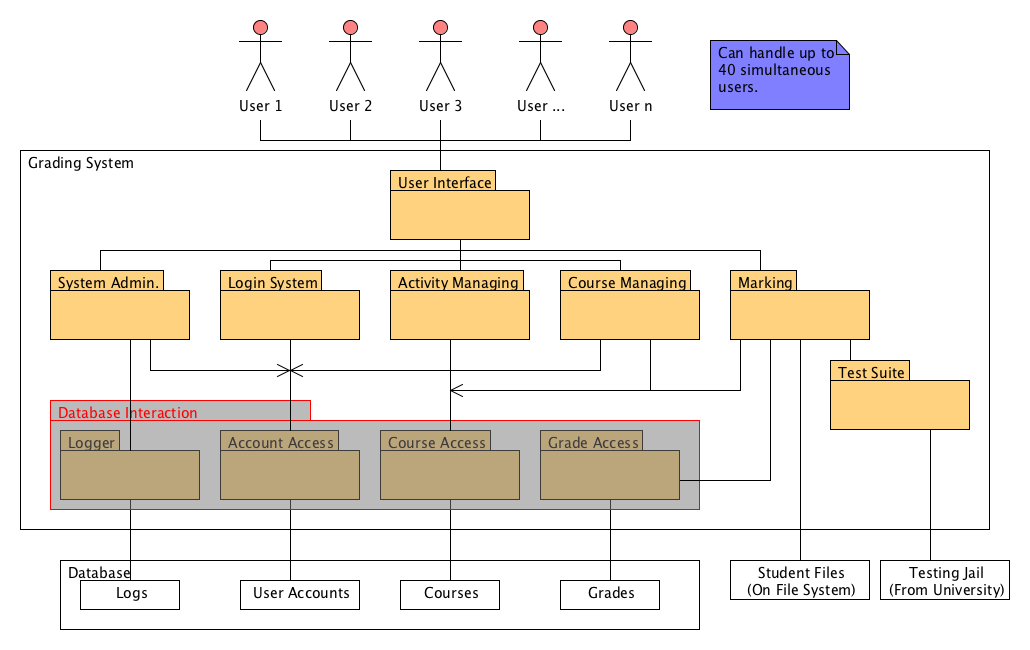
\includegraphics[scale=0.55]{../images/architectureDiagram}}

\subsection{Sub-system Descriptions}
\subsection{Refined Use Cases}
\textbf{Use Case Name: testCourse (\#3.9)}\\
\textbf{Scenario:}
TA Marker Joe Fresh runs the test suite to grade Student Tina Turner’s “Assignment 4” 
code.\\
\textbf{Preconditions:}
\begin{itemize}
	\item Joe has logged in successfully.
	\item Joe has navigated to the “Marking” page for Assignment 4. (\textbf{Marking 
		$\rightarrow$ Courses $\rightarrow$ Select Activity $\rightarrow$ Assignment 4}).
	\item The test suite  and database are ready to be initialised.
	\item Tina has turned in Assignment 4, and her code can be compiled.
\end{itemize}
\textbf{Main Flow of Events:}
\begin{enumerate} 
	\item Joe clicks on the “Test Code” button in the bottom right corner of the screen.
	\item The program will compile and run Tina’s  code.
	\item Assuming the code generates output, an output file is generated.
	\item The screen will change to the “Test Suite” page, displaying the output 
		generated code, the solution code and a diff (the differences between the 
		two documents) of the two outputs.
	\item Joe will look at the diff, then the solution code and mark the output by
		tabbing between the test suite and the rubric.	
	\item Additionally, Joe may comment on Tina’s code by 	clicking the “Submit 
		Comment” button.
	\item Joe finishes marking and clicks “Submit”.
\end{enumerate}
\textbf{Postconditions:}
\begin{itemize}
\item The program saves the grade to the database. 
\item Joe is returned to the “Select Activity” page for Assignment 4.
\end{itemize}
\textbf{Exceptional Flow of Events:}
\begin{enumerate}
 	\item If the compiled code doesn’t generate output, or crashes from a runtime 
 		error, then a message will appear in the “Student Solution” field saying that  
 		no output could be generated.
	\item If the rubric is not completely filled out (i.e. one or more of the items in the 
		rubric that do not have a mark)
\end{enumerate}
\textbf{Use Case Name: createActivity (\#x.x)} \\
\textbf{Scenario:} Instructor John Smith creates an activity “Assignment 1” to his
course CMPT 165.\\
\textbf{Preconditions:}
\begin{itemize}
	\item John has successfully logged in to the system.
	\item John is the instructor of CMPT 165 and it exists in the courses database.
	\item The system is at its initial screen after John's login.
\end{itemize}
\textbf{Main Flow of Events:}
\begin{enumerate}
	\item The use case starts when John selects the "Activity Management" button.
	\item John then chooses to "Add An Activity" which sends him to a page listing
		the courses he is currently teaching.
	\item John then selects CMPT 165 from his list of courses to add an activity to, and is sent to 	
		a page containing fields to enter all the necessary details of an activity.
	\item  John inputs the necessary details for "Assignment 1" into the fields for them. These
		fields are:
	\begin{enumerate}
		\item Name of activity
		\item Activity description
		\item Type of activity
		\item Language of activity
		\item Group or individual activity
		\item Solution
		\item Rubric
		\begin{enumerate}
			\item 	John presses the "Rubric" tab.
			\item John enters the description of the aspect being graded, and the 
					possible grade for that aspect.
			\item The above process (ii.) is repeated for as many rubric aspects as desired
					(possibly none).
			\item John presses "Save" and the rubric is added to the activity.
					A message is displayed confirming the rubric has been added successfully.
			\item John is returned to the form for details of the activity.
		\end{enumerate}
		\item Due date with penalties/bonuses
			\begin{enumerate}
				\item John enters a due date for the submission.
				\item John can optionally add additional due dates with mark penalties or
					bonuses based off of the additional due dates.
			\end{enumerate}
		\item Test input and output files (for coding activities only)
			\begin{enumerate}
				\item John presses "Attach Test Input/Output".
				\item John is prompted to enter the locations of any testing input
					files, as well as the locations of solution output files for a specific
					input. 
				\item John confirms the file attachment and the file is added to the form of
					the activity.
			\end{enumerate}
	\end{enumerate}
	\item The instructor presses the "Finish" button.
	\item The system verifies that the details entered for the activity are valid in every field.
	\item A message is displayed confirming that the activity details were correct and the
		activity has been added to the course.
	\item The system returns John to his initial screen.
	\item The use case terminates once John has been returned to the initial
		screen.
\end{enumerate}
\textbf{Postconditions:}
\begin{itemize}
	\item The system has saved "Assignment 1" in the database for CMPT 165.
	\item The system has returned to John's initial screen.
\end{itemize}
\textbf{Exceptional Flow of Events:}
\begin{enumerate}
	\item \underline{Details for activity are not complete:} If John did not specify
			all the necessary details for creating an activity, a message will be displayed
			stating which fields were empty when John attempted to confirm.
			He will remain on the form for the activity, and be prompted to fill in necessary
			fields.
	\item \underline{Invalid data for a field of the activity:} If John enters invalid
			data for one of the details of the assignment, a message will be displayed
			specifying which field contained invalid data. He will remain on the form and
			be prompted to correct errors in his entries.
\end{enumerate}

\section{Low Level Design}
\subsection{Interaction Diagrams}
\textbf{Collaboration Diagram (testCourse):}\\
\centerline{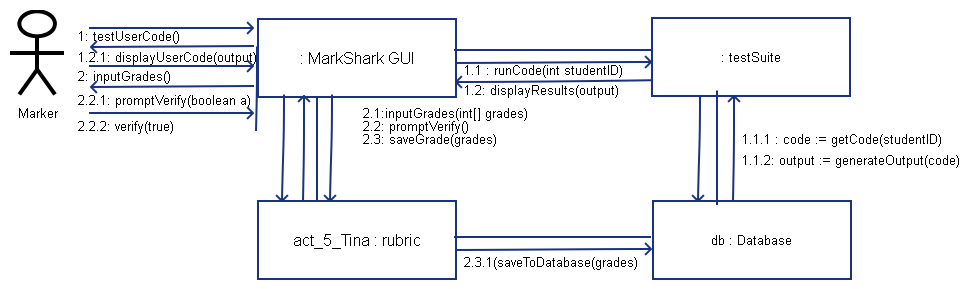
\includegraphics[scale=0.5]{../images/designDocImages/Collaboration_Diagram_Use_Case.png}}
\clearpage
\textbf{Sequence Diagram (createActivity):}\\
\centerline{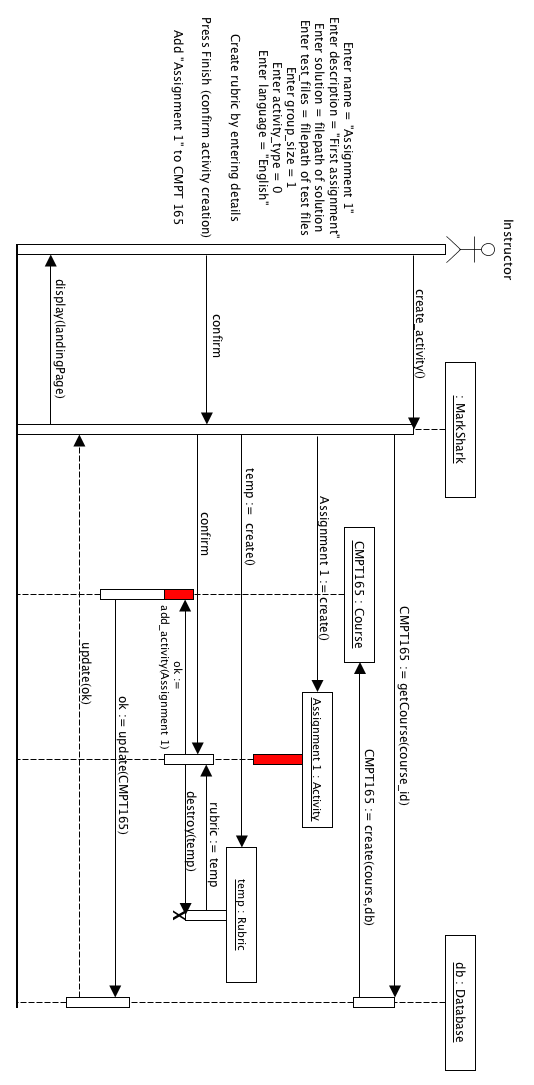
\includegraphics[scale=0.55]{../images/designDocImages/sequenceDiag.png}}
\subsection{Class Diagram}
\centerline{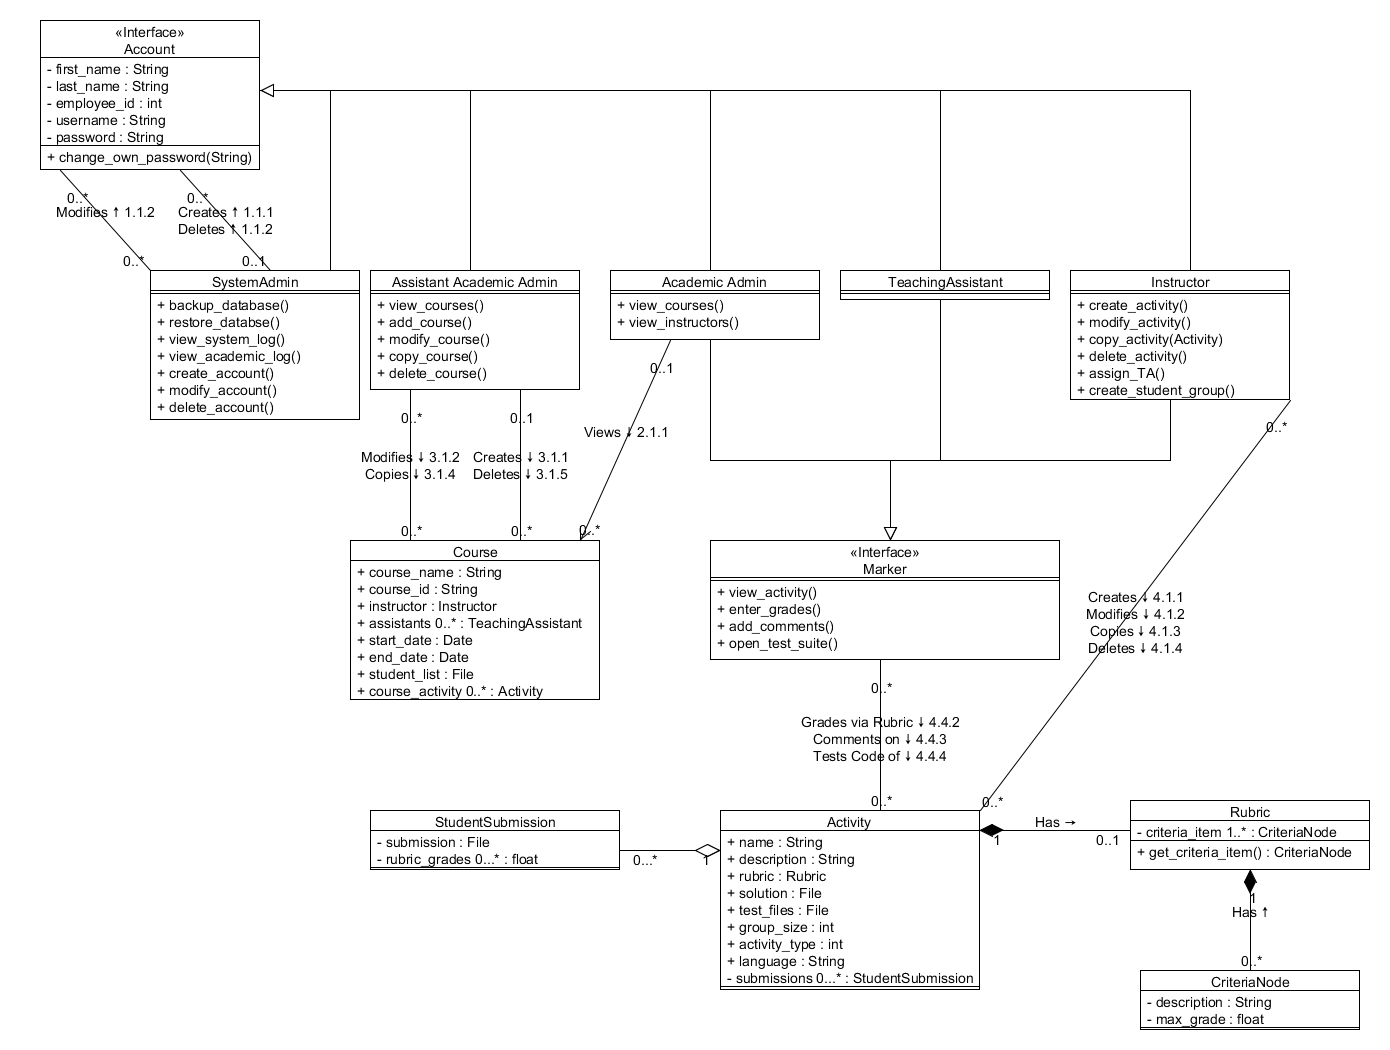
\includegraphics[scale=0.5]{../images/Class_Diagram_Detailed}}

\section{Data Persistence}

\centerline{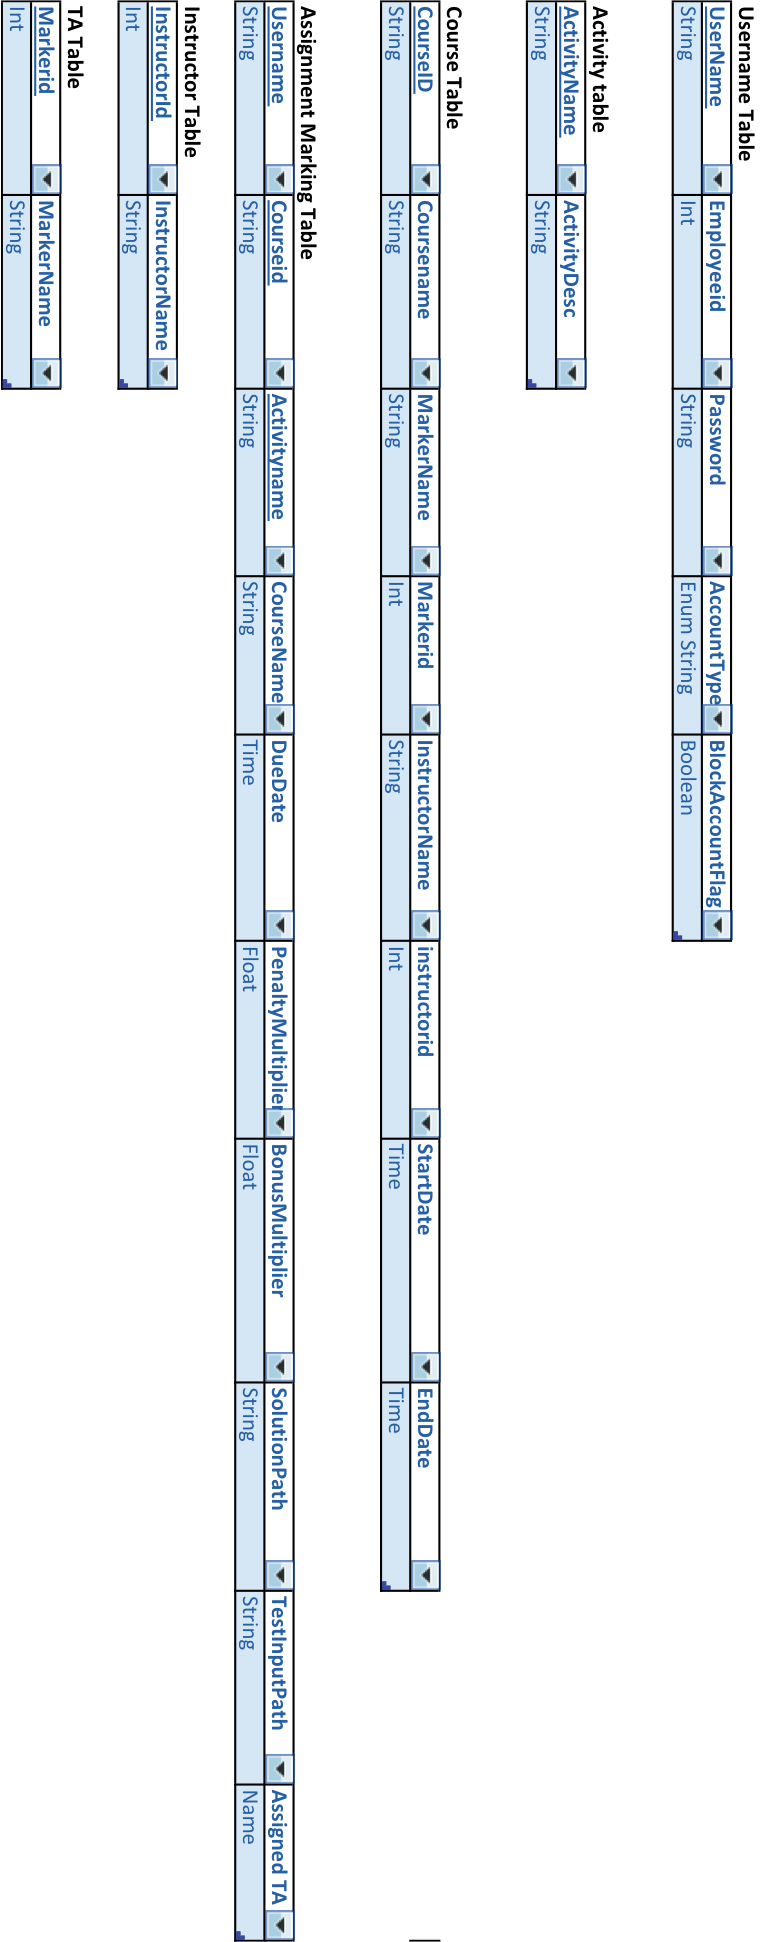
\includegraphics[scale=0.5]{../images/Data_Persistance.png}}


\end{document}
